% Chapter Template

\chapter{Introduction}\label{chapter:firstchapter} % Main chapter title

\label{Chapter1} % Change X to a consecutive number; for referencing this chapter elsewhere, use \ref{ChapterX}

%----------------------------------------------------------------------------------------
%	SECTION 1   % TARGET 1500 WORDS IN THIS CHAPTER
%----------------------------------------------------------------------------------------

\section{An Overview}
%% some background on the importance and relevance of universal design
%% explain the issue that needs to be addressed using this concept
%% mention this is a new project
%% frame this around a gap statement
\subsection{Disabilities affect many people}
In today's day and age where humans are living longer than ever before, the very young, elderly and people with a disability is a demographic that is constantly growing as populations increase.
In Australia, where this project is based, the current population of people with a disability represents an estimation of 1 in 6 people \cite{ausstats}, a group that is far more common than many may realise.
This has indirectly led to the concept of Universal Design (UD), established at North Carolina State University by Dr Ronald Mace, to make designs accessible to all people, regardless of age or disability \cite{ronald}.
The term ‘Universal Design’ is a concept first coined by Ron Mace where “the design of products, environments, programmes and services to be usable by all people, to the greatest extent possible, without the need for adaptation or specialized design” \cite{nda}. 

\subsection{Digital Sovereignty and Capability Maintenance of accessibility features} %%look up and add capability maintenance
On a different yet related note, individuals are losing out on the right to repair, modify and maintain their own electronic devices, as the everpresent concept of planned obsolescence continues to dominate the market due to the undeniable profitability of doing so \cite{obsolescence2}.
%Factors such as increased complexity of computer systems and the desire of companies to protect their intellectual property, mean that true Digital Sovereignty is unrealistic. %%%CONTRADICTORY
This problem threatens the Digital Sovereignty (DS) movement, which has opened an avenue for the 'MEGAphone' as a truly open and secure mobile device overseen by Dr Paul Gardner-Stephen \cite{mobilehistory}.
The MEGAphone is based on a project developed by the Museum of Electronic Games and Arts (MEGA), to bring life to the never released Commodore65 computer \cite{mega65}.

Gardner-Stephen's goal is to provide users with a secure mobile device, built on a far less complex and therefore more transparent computer system than modern alternatives, of which the ability repair, modify and maintain remains the user's right.
As manufacturers continue to design their products with increasingly shorter lifespans, this can make life difficult, especially for people with a disability as their devices will cease to receive system updates much sooner, resulting in less security and quicker loss of capability.
More recently, Gardner-Stephen and Nabben \cite{capability} have looked into how the MEGAphone can be used in disaster situations, by partnering with the 'Serval Project' \cite{serval} as a device that can be maintained and retain full network capability in situations where it is most crucial.

\subsection{Motivation for this project} \label{Motivation}
The purpose of this project is to provide enhanced telephony access to everyone, regardless of physical impairments, or age.
The concept of UD will be employed to develop a truly accessible MEGAphone for all users.

The 'seven design principles' are a set of design guidelines developed by Molly Follette Story at the 'Center for Universal Design' located in North Carolina State University \cite{sevenprinciples}.
These principles are vital to the success of this project, as not only does this provide more clarity into the development of an accessible design but also a method in which to grade the accessibility of said design.
This will be achieved while staying true to the DS movement by continuing to provide users with a platform that they can easily maintain, modify and repair.

\subsection{Goals of this project} \label{Goals}
The MEGAphone housing deliverable (otherwise referred to as a 'case' or 'chassis') is an entirely new project, based on existing PCB constraints, which is important to define as UD is an iterative process and therefore must be at the centre of the design philosophy from the start \cite{incldesign}.
The aim is to create an entirely new accessible case for the current revision of the project, supported by the aforementioned seven design principles.

This project will require computer-aided design (CAD) 3D modelling software in order to successfully translate concept sketches into a real tangible design.
Another requirement will include electronic design software, to design the accompanying PCBs for this project as there will be a requirement to adapt to the existing constraints of the MEGAphone PCB.
The third requirement will be the use of Xilinx's Vivado FPGA programming software in order to design an accessible user interface (UI) that allows users to interact with an external digital input device.

% Accessible design practices will play a central role in the design process as the success of the final product depends on its ability to provide accessibility to all (regardless of age or disability). 
As mentioned, this project does have existing constraints, in that it is adapted around an existing PCB, however, this design will take the opportunity to uphold the aforementioned design philosophy.
While a completely new PCB design is implausible at this stage, this project will make the note to include a proposed re-design of the MEGAphone PCB following these design practices.
Additionally, this project will look into the relationship that UD and DS share so that users can not only have an easily accessible interface, but one that satisfies the open and transparent philosophy of DS.
%% planned ob works against people with a disability, capability maintenance

%----------------------------------------------------------------------------------------
%	SECTION 2
%----------------------------------------------------------------------------------------
\section{Background on the MEGAphone}

%% how was this project formed, and who works on it
The ‘MEGAphone’ is a digitally sovereign mobile device created by Dr Paul Gardner-Stephen with the intent to promote Digital Sovereignty \cite{mobilehistory}.
This project began when a trend was noticed in modern consumer electronics, a trend that still exists today, in that companies design their products with ‘planned obsolescence’ in mind.
Gardner-Stephen believes that users should have the ability to repair or modify any aspect of their device without difficulty \cite{mobilehistory}.

\begin{figure} [h]
    \centering
    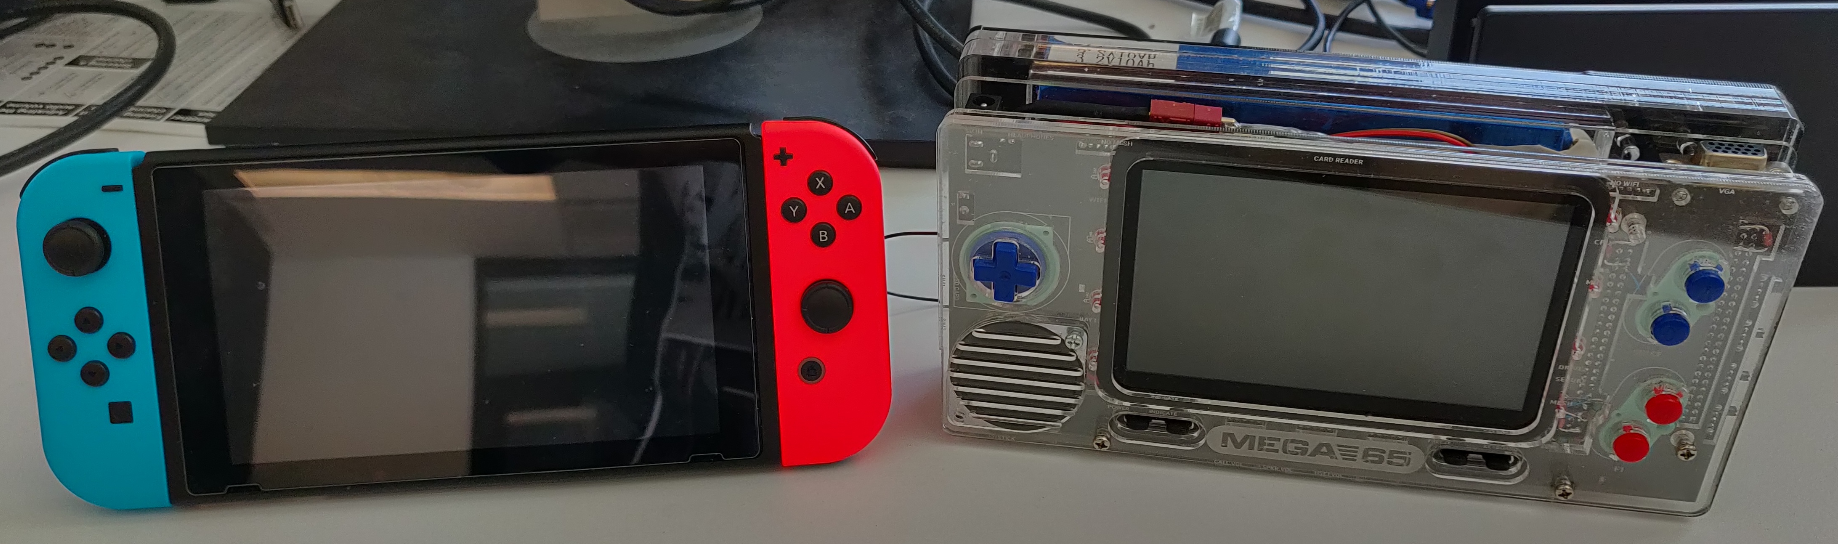
\includegraphics[width=12cm,height=10cm,keepaspectratio]{Figures/megaphone.png}
    \caption{On the right is the first revision of the MEGAphone device. On the left, a Nintendo Switch \cite{nintendoswitch} can be seen as a size comparison for the MEGAphone.}
    \label{fig:Jellybean}
\end{figure}

%% explain the purpose of FPGA, and security features
The MEGAphone incorporates the use of a field-programmable gate array (FPGA), which acts as a sort of hardware programmable CPU designed to mimic the architecture of the unreleased Commodore65.
This eliminates the costly alternative of emulation and provides the option for modern performance advancements in aspects such as storage and boot time.
One of the marketable assets of this project is that due to the simplicity of the system, the device is very secure.
This coupled with the addition of hardware power switches, gives users the peace of mind that insecure wireless modules cease to operate when they are switched off and not only trust that this is the case.
% (Section \ref{sec:firstsection}).

%----------------------------------------------------------------------------------------
%	SECTION 3
%----------------------------------------------------------------------------------------
\section{Project Objectives} \label{Objectives}

The main objective of this project is to design a prototype case for the MEGAphone that follows the seven principles of UD, established at the Center for Universal Design, North Carolina State University \cite{sevenprinciples}. 
Other deliverables will be in support of this case and will include, PCBs to assist with add-on features and hardware-implemented accessibility features in the FPGA.

This thesis will document the entire design process including any modifications to the designs, along with justifications as to why specific changes were made as opposed to any logical alternatives.
In terms of the research component, this thesis aims to address the relevance of UD in the design process as well as identifying the importance of device sovereignty and how it can be supported during this process.

Specifically, this thesis will look into the history of UD, provide some examples of how certain features have been implemented in existing products and how the effects of the COVID-19 pandemic have negatively affected this project.
One aspect that was affected by the pandemic was the plan to hold focus groups (for people with a disability), to provide feedback on the design at each iteration.
Instead, the feedback received during this project was solely from industry professionals due to valid health concerns from Novita \cite{novita}, the organisation that was likely to host these meetings.

The desired output of this project as documented will be at least one physical prototype of the MEGAphone case and supporting components as well as hardware-implemented accessibility features for the MEGA65 OS.
Multiple physical prototypes of this project will allow for not only a demonstration of the UD features but also a demonstration of the iterative process of engineering design.

%----------------------------------------------------------------------------------------
%	SECTION 4
%----------------------------------------------------------------------------------------
\section{Research Questions}

This thesis aims to answer multiple research questions:

\begin{enumerate}
    \item What is the relationship between Digital Sovereignty and Universal Design?
        \begin{enumerate}
        \item[-] This project should establish how UD and DS can be used to make a mobile device that not only satisfies both concepts but actively shows how they can be mutually beneficial.
        \end{enumerate} 
    \item Why is Universal Design important in the design of products today?
        \begin{enumerate}
        \item[-] Support the concept that UD should be used in any design project, as it benefits all users to a greater extent.
        \end{enumerate}
    \item Why is Digital Sovereignty important in the design of electronic products today?
        \begin{enumerate}
        \item[-] Show how DS is important to individuals with their electronics as it protects their right to a secure and open platform.
        \end{enumerate} 
    \item How can the seven design principles be used in the design of the MEGAphone case to support those with disabilities?
        \begin{enumerate}
        \item[-] Demonstrate how these seven design principles apply to the accessibility of the MEGAphone housing concept.
        \end{enumerate} 
    \item How can the 'Right to Repair' philosophy be used in support of the universally designed MEGAphone case?
        \begin{enumerate}
        \item[-] Demonstrate how the MEGAphone concept can be made easier to repair and maintain.
        \end{enumerate} 
    \item What are the effects of COVID-19 on Digital Sovereignty and Universal Design regarding the MEGAphone project?
        \begin{enumerate}
        \item[-] Discuss the importance of end-user input in the design of the MEGAphone concept and how COVID-19 affects that ability.
        \item[-] Discuss why sovereign devices are important in disaster scenarios and to those with a disability.
        \end{enumerate} 
\end{enumerate}

%----------------------------------------------------------------------------------------
%	SECTION 5
%----------------------------------------------------------------------------------------
\section{Scope of Project}

This project will look at the history and importance of UD and DS in the design of products today as well as the relationship between those two concepts.
The development of a unique, universally designed chassis prototype graded against the seven design principles \cite{sevenprinciples} will be presented, along with multiple PCB designs that support features of the housing.
The existing MEGAphone PCB and hardware-implemented accessibility features written in VHDL for the MEGA65 OS will also be presented.

In terms of what is considered out of scope, the main MEGAphone PCB or 'motherboard' itself will remain untouched, meaning that any changes will be external, either in the form of new PCBs or new components.
Additionally, any software running on the MEGAphone, such as in C code, is also considered out of scope.

It is important to distinguish that VHDL is a hardware description language, which does not actually affect the software side of things, hence is in scope.
To the author's best knowledge, this is the first digitally sovereign smartphone project with an emphasis on being universally designed.
%% possible update, revise this at some point
%% what is out of scope? software out of scope etc

% %----------------------------------------------------------------------------------------
% %	SECTION 6
% %----------------------------------------------------------------------------------------
\section{Contributions to the Field} %% past tense!

The MEGAphone device is a platform that exists to provide people with true control over their data, and by extension their right to repair, modify and maintain their device.
This project aims to support the MEGAphone project by developing an interface that enhances the accessibility of the device.
The author believes that a unique project such as the MEGAphone, with the ability to give users a secure and truly open telephony platform, should be accessible to everyone regardless of their age or ability.
This thesis investigated exactly how that could be achieved in order to deliver a MEGAphone device chassis, supporting existing PCBs and hardware-implemented user interface that embodies the vision of UD and DS.\vspace{5mm}

Specifically, a breakdown of the author's contributions to the field are:
\begin{enumerate}
    \item An examination of the relationship between Digital Sovereignty and Universal Design.
    \item Analysis of the existing MEGAphone PCB design from the perspective of UD.
    \item The creation through iteration of a UD housing for the MEGAphone PCB.
    \item The improvement of the MEGAphone device layout to improve its UD properties.
    \item The design of practical modifications to the MEGAphone PCB design that allows the majority of the UD improvements to be realised, without requiring a complete and costly re-design of the MEGAphone PCB.
    \item The proposal of further improvements to the MEGAphone PCB and case designs to further improve their UD properties.
    \item The creation of a MEGAphone device prototype, including UD features and housing, that can be used in future UD studies of the MEGAphone.
\end{enumerate}

%----------------------------------------------------------------------------------------
%	SECTION 7
%----------------------------------------------------------------------------------------
\section{Structure of Thesis}

This thesis is organised as follows:
\begin{itemize}
    \item Chapter \ref{Chapter1} addresses the aims of the project, provides some context on the MEGAphone, lists the research questions and contributions of the author.
    \item Chapter \ref{Chapter2} investigates how Universal Design can help to overcome many issues in product design that people with disabilities face without the need for specialized equipment. Additionally, the lack of Digital Sovereignty in electronics devices is addressed as well as how it affects the user and the sovereignty of their device in disaster situations.
    \item Chapter \ref{Chapter3} focuses on the methods and tools used to plan, design and manufacture this project.
    \item Chapter \ref{Chapter4} details the iterative design process and the incremental changes made to the design, toward a definitive prototype, with justifications as to why each feature was implemented.
    \item Chapter \ref{Chapter5} reviews the final 3D-printed prototype and presents some changes in response to the outcome.
    \item Chapter \ref{Chapter6} provides concluding remarks as well as a final evaluation of the case prototype, PCBs, hardware-implemented 'software' features thereby suggesting future work to be undertaken.
\end{itemize}